% ══════════════════════════════════════════════════════════════════
\chapter{Results}
\label{ch:results}

This chapter reports the numerical results obtained by applying the
four computational strategies of \cref{ch:framework} to the
spin-dependent charmonium Hamiltonians of \cref{ssec:matrices}: exact
diagonalisation (classical reference), VQE in the direct (2-qubit) and
Jordan--Wigner (4-qubit) encodings, VQITE, and TTITE. We first run a
noiseless sanity check on a simulator (\cref{sec:noiseless}), then
re-execute the same protocols under depolarising noise to characterise
the resilience of each method (\cref{sec:noisy}). A brief summary
(\cref{sec:results-summary}) closes the chapter.

% ──────────────────────────────────────────────────────────────────
\section{Experimental setup}
\label{sec:results-setup}

All quantum computations run through Qiskit's
\texttt{AerSimulator}. Pauli expectation values are
estimated with $N_{\mathrm{shots}} = 8192$ shots per term; VQITE
overlaps for the metric tensor use $4\!\times\! N_{\mathrm{shots}}$. The
classical optimiser for VQE is COBYLA with a maximum of $300$
iterations. VQITE uses $40$ forward-Euler imaginary-time steps with
$\Delta\tau = 0.05$ and Tikhonov regularisation $\lambda = 10^{-3}$.
TTITE uses total imaginary time $\tau_{\mathrm{total}} = 5$ with step
$\Delta\tau = 0.02$ and Taylor order $R = 10$. The depolarising channel
of \cref{eq:depolarizing} is applied to every gate when the noisy
backend is in use; rates swept are
$p \in \{0.0, 0.005, 0.01, 0.02, 0.05\}$ with three independent repeats
per configuration. A random seed (42) makes the runs reproducible. All
energies below are reported in inverse-femtometres; multiplication by
$\hbar c = 197.326$~MeV$\cdot$fm converts to MeV.

The full implementation---including the Hamiltonian builders, the three
algorithm wrappers, the noise sweep driver, and the standalone
visualisation script that produces every figure in this chapter---is
released as open-source software at
\url{https://github.com/Lucas-Froguel/quarkonium-simulations}~\cite{froguel_quarksim},
together with all configuration files needed to reproduce the runs
reported below.

% ──────────────────────────────────────────────────────────────────
\section{Noiseless benchmark}
\label{sec:noiseless}

\subsection{Ground-state energies}
\label{ssec:noiseless-ground}

\Cref{tab:noiseless} reports the ground-state energy of each channel
obtained by each method, alongside the exact diagonalisation reference.
\Cref{fig:convergence} shows the corresponding energy convergence
traces: COBYLA iterations for VQE, imaginary-time steps for VQITE,
Trotter segments for TTITE.

\begin{table}[htbp]
\centering
\caption{Ground-state energies in the noiseless simulator
  ($p = 0$). Energies in fm$^{-1}$; absolute errors are
  $\Delta E = |E_{\mathrm{est}} - E_{\mathrm{exact}}|$. ``VQE'' uses
  the direct encoding (2 qubits); ``VQE-JW'' uses the Jordan--Wigner
  encoding (4 qubits, UCC ansatz). $\mathcal{F}$ is the fidelity with
  the exact ground state.}
\label{tab:noiseless}
\renewcommand{\arraystretch}{1.15}
\small
\begin{tabular}{llrrrr}
\toprule
Channel & Method   & $E_{\mathrm{est}}$ & $E_{\mathrm{exact}}$ & $\Delta E$  & $\mathcal{F}$ \\
\midrule
\multirow{4}{*}{${}^1S_0$}
        & VQE      & $0.452$ & $0.391$ & $0.060$ & $0.975$ \\
        & VQE-JW   & $0.419$ & $0.391$ & $0.027$ & $0.989$ \\
        & VQITE    & $0.376$ & $0.391$ & $0.016$ & $0.99995$ \\
        & TTITE    & $0.419$ & $0.391$ & $0.027$ & $0.99984$ \\
\midrule
\multirow{4}{*}{${}^3S_1$}
        & VQE      & $0.769$ & $0.752$ & $0.017$ & $0.991$ \\
        & VQE-JW   & $0.735$ & $0.752$ & $0.017$ & $0.993$ \\
        & VQITE    & $0.744$ & $0.752$ & $0.008$ & $0.99990$ \\
        & TTITE    & $0.770$ & $0.752$ & $0.018$ & $0.99989$ \\
\midrule
\multirow{4}{*}{${}^1P_1$}
        & VQE      & $2.780$ & $2.781$ & $0.001$ & $0.998$ \\
        & VQE-JW   & $2.745$ & $2.781$ & $0.036$ & $0.999$ \\
        & VQITE    & $7.416$ & $2.781$ & $4.635$ & $0.169$ \\
        & TTITE    & $2.785$ & $2.781$ & $0.003$ & $0.99998$ \\
\bottomrule
\end{tabular}
\end{table}

\begin{figure}[htbp]
\centering
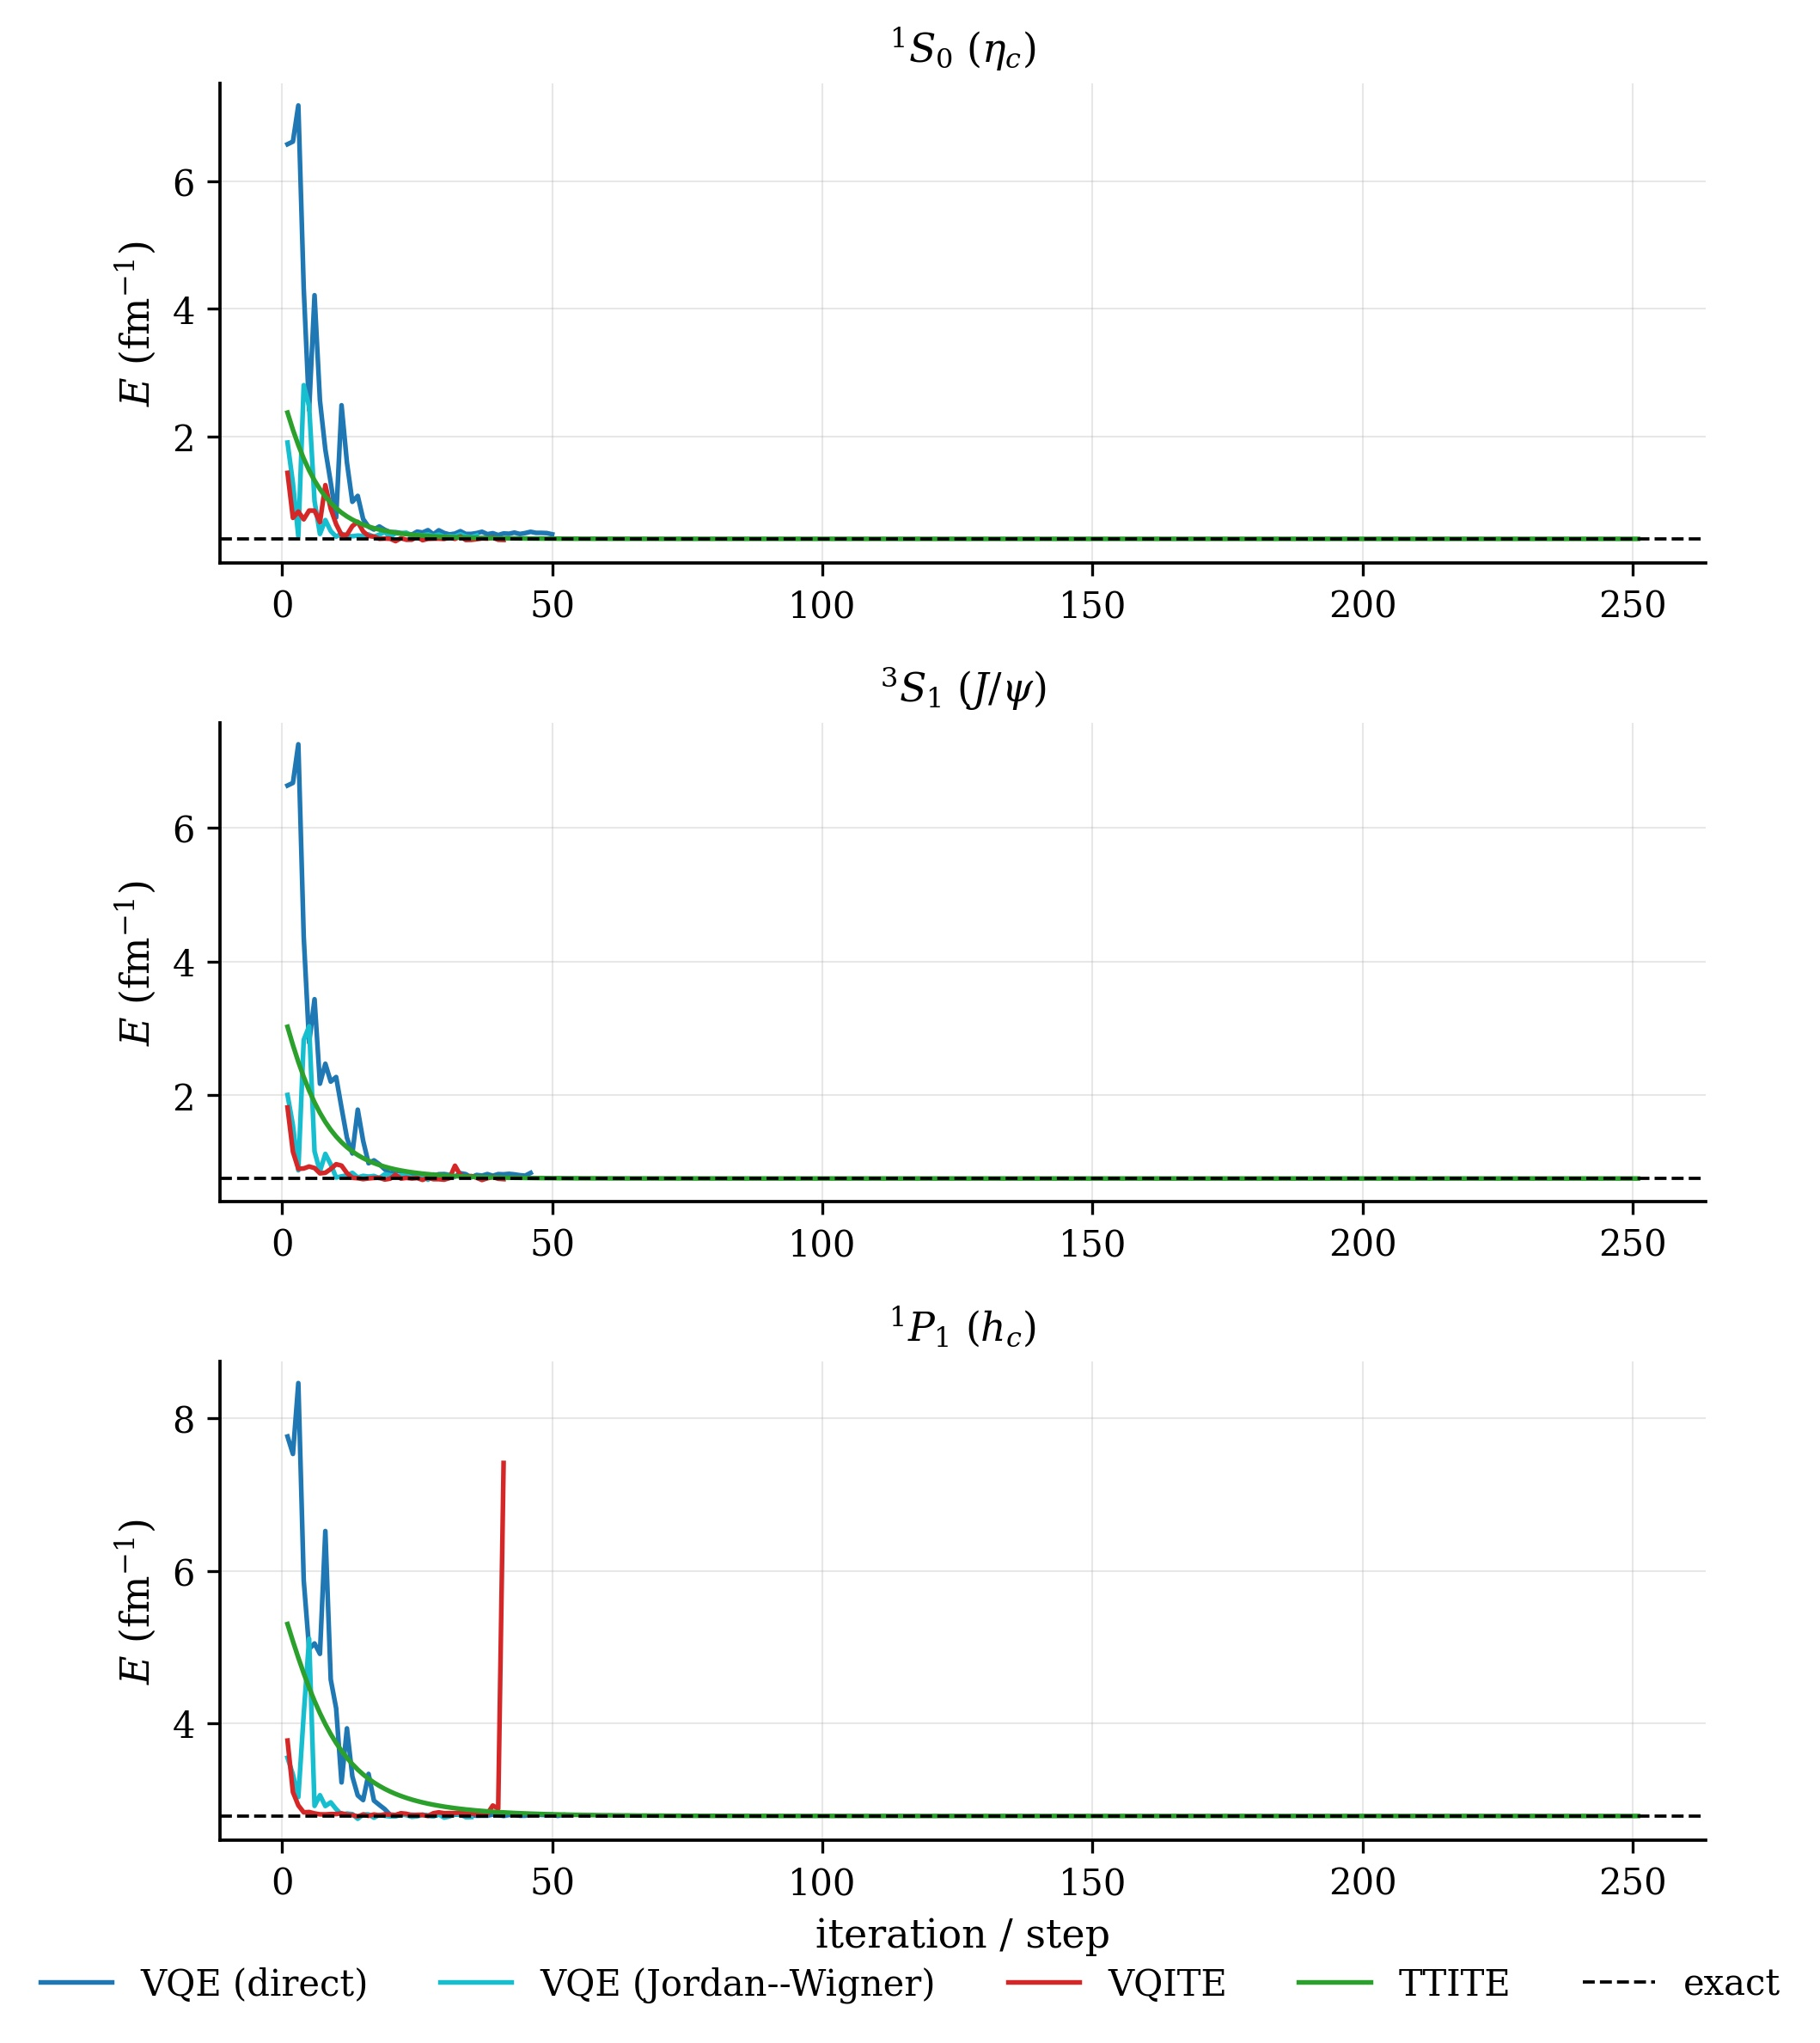
\includegraphics[width=\textwidth]{figures/convergence.jpeg}
\caption{Noiseless energy convergence on each channel. The horizontal
  dashed line marks the exact eigenvalue. The $x$-axis is the COBYLA
  iteration for VQE/VQE-JW, the imaginary-time step for VQITE, and the
  Trotter segment for TTITE.}
\label{fig:convergence}
\end{figure}

Three patterns emerge. First, TTITE consistently produces a
high-fidelity ground state (\,$\mathcal{F} \gtrsim 0.9999$ on every
channel), reflecting the fact that the algorithm does not depend on
ansatz expressibility; its $\mathcal{O}(10^{-2})$~fm$^{-1}$ energy
error is dominated by the shot-noise estimator of the final
expectation value rather than by any algorithmic bias. Second, the
two VQE variants agree to within $\sim 10^{-2}$~fm$^{-1}$ across all
channels, confirming that the Jordan--Wigner encoding faithfully
reproduces the physics encoded by the direct mapping. Third, VQITE is
the most volatile of the three: on ${}^1S_0$ and ${}^3S_1$ it
recovers the true ground state with fidelity above $0.9999$, but on
${}^1P_1$ the local McLachlan descent on the three-parameter
manifold falls into an unphysical region (final energy $7.42$, well
above any low-lying eigenvalue, fidelity $\sim 0.17$). The failure is
a known sensitivity of VQITE to the initial parameter point and to
shot noise on the quantum metric estimate; VQE on the same ansatz is
not similarly trapped because COBYLA samples a trust region and can
escape such basins.

\subsection{Ground-state error summary}
\label{ssec:noiseless-summary}

\Cref{fig:energy_summary} collects the absolute errors of
\cref{tab:noiseless} into a single bar chart, separating the
$\sim 10^{-3}$ accuracy of TTITE from the $\sim 10^{-2}$ ansatz-limited
accuracy of the variational methods.

\begin{figure}[htbp]
\centering
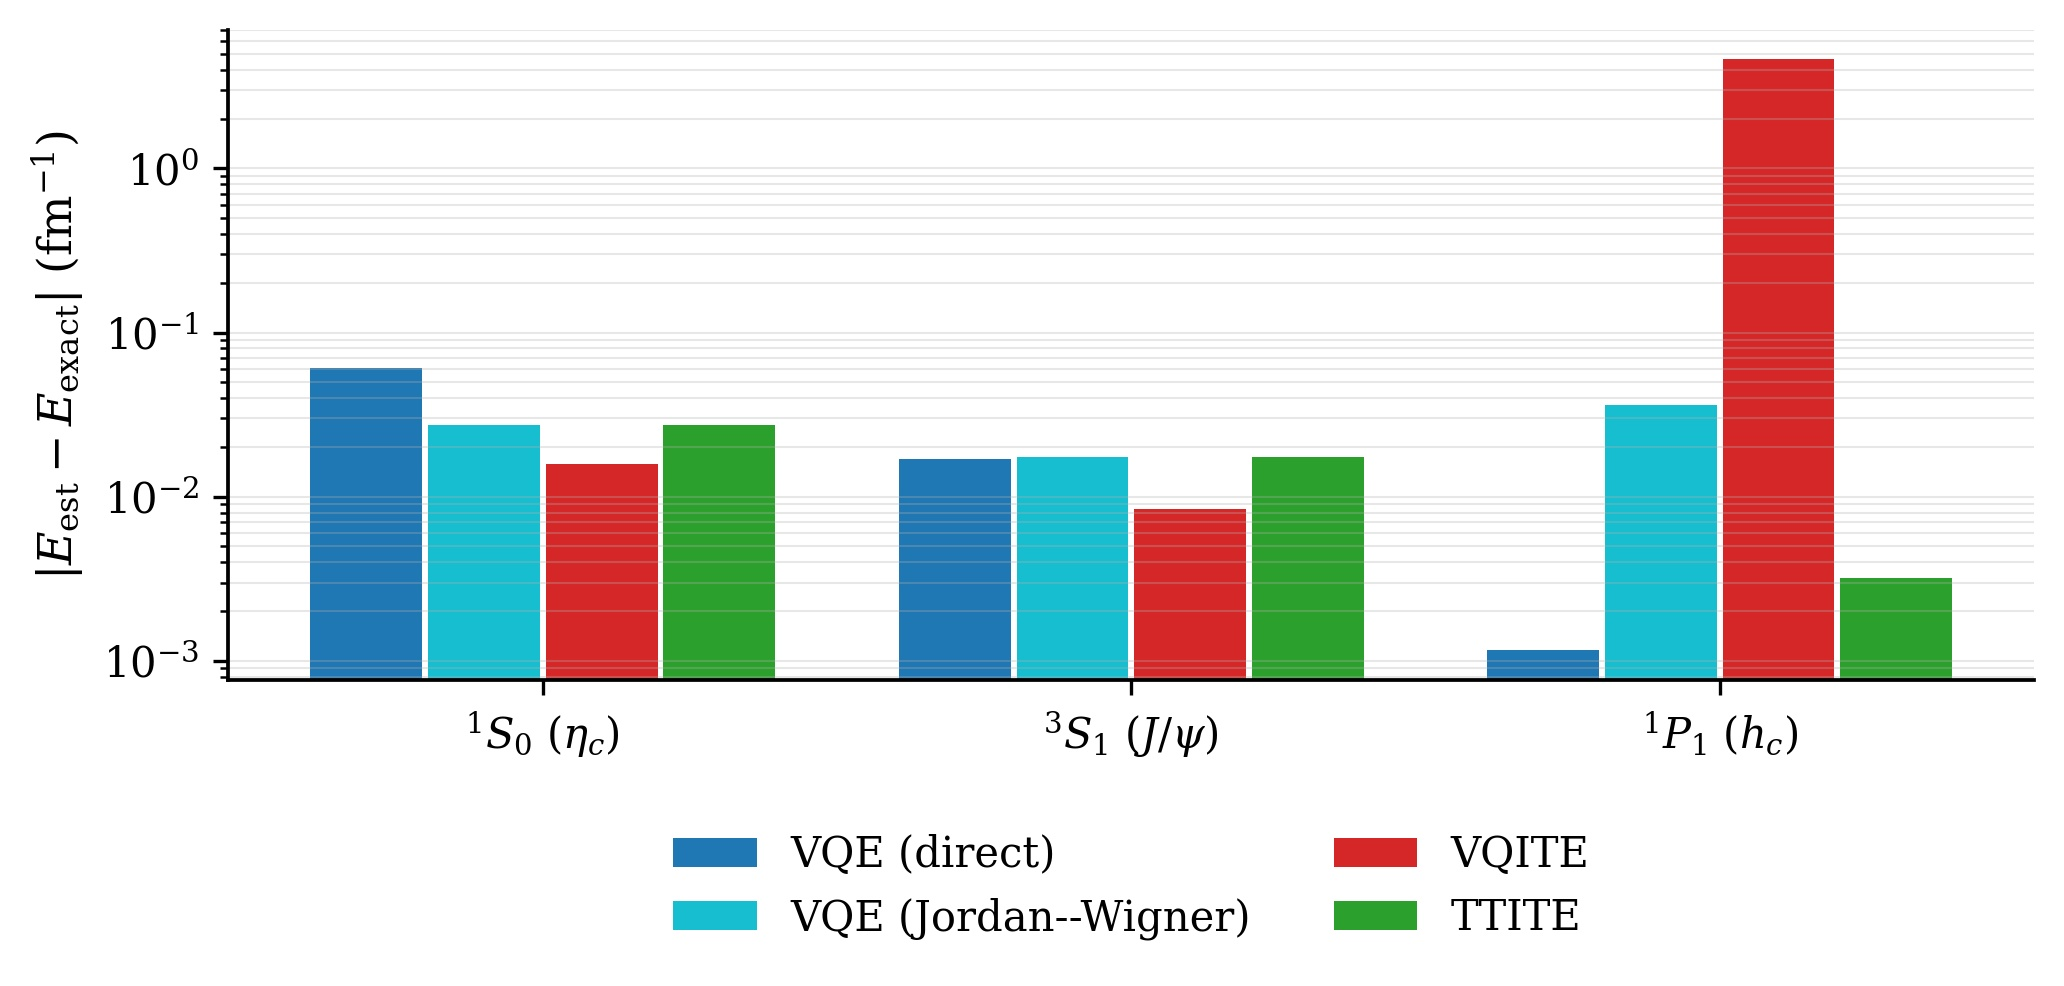
\includegraphics[width=0.85\textwidth]{figures/energy_summary.jpeg}
\caption{Absolute ground-state energy error per (channel, method) in the
  noiseless simulator (log scale). TTITE saturates the simulation
  precision; the variational methods are bounded above by their ansatz
  expressibility.}
\label{fig:energy_summary}
\end{figure}

\subsection{Excited states}
\label{ssec:excited}

We compute the four lowest eigenvalues per channel using the
orthogonalisation/penalty strategy of \cref{ssec:vqe_excited}. Both
VQE encodings are run; the VQITE column of \cref{tab:excited} is
reserved for follow-up work---the same penalty machinery
(\cref{eq:penalised_H}) applies, but the per-step circuit overhead
makes a full sweep impractical within the time budget of this thesis.
TTITE does not support excited states directly and is omitted from
this table.

\begin{table}[htbp]
\centering
\caption{Ground and excited-state energies (fm$^{-1}$) obtained by
  penalty-based VQE. $E_{\mathrm{exact}}$ is the eigenvalue of the
  classical $4\times 4$ diagonalisation. ``--'' entries are reserved
  for VQITE, which is left for future work.}
\label{tab:excited}
\renewcommand{\arraystretch}{1.15}
\small
\begin{tabular}{llrrrr}
\toprule
Channel & $k$ & $E_{\mathrm{exact}}$ & VQE     & VQE-JW  & VQITE \\
\midrule
\multirow{4}{*}{${}^1S_0$}
& $0$ & $0.391$ & $0.429$ & $0.472$ & --- \\
& $1$ & $3.483$ & $3.489$ & $3.466$ & --- \\
& $2$ & $5.643$ & $5.573$ & $5.519$ & --- \\
& $3$ & $7.545$ & $7.048$ & $7.509$ & --- \\
\midrule
\multirow{4}{*}{${}^3S_1$}
& $0$ & $0.752$ & $0.808$ & $0.776$ & --- \\
& $1$ & $3.633$ & $3.656$ & $3.678$ & --- \\
& $2$ & $5.727$ & $7.458$ & $5.927$ & --- \\
& $3$ & $7.646$ & $5.660$ & $6.179$ & --- \\
\midrule
\multirow{4}{*}{${}^1P_1$}
& $0$ & $2.781$ & $2.798$ & $2.772$ & --- \\
& $1$ & $4.883$ & $4.889$ & $4.923$ & --- \\
& $2$ & $6.756$ & $7.882$ & $6.779$ & --- \\
& $3$ & $8.770$ & $7.058$ & $5.613$ & --- \\
\bottomrule
\end{tabular}
\end{table}

\begin{figure}[htbp]
\centering
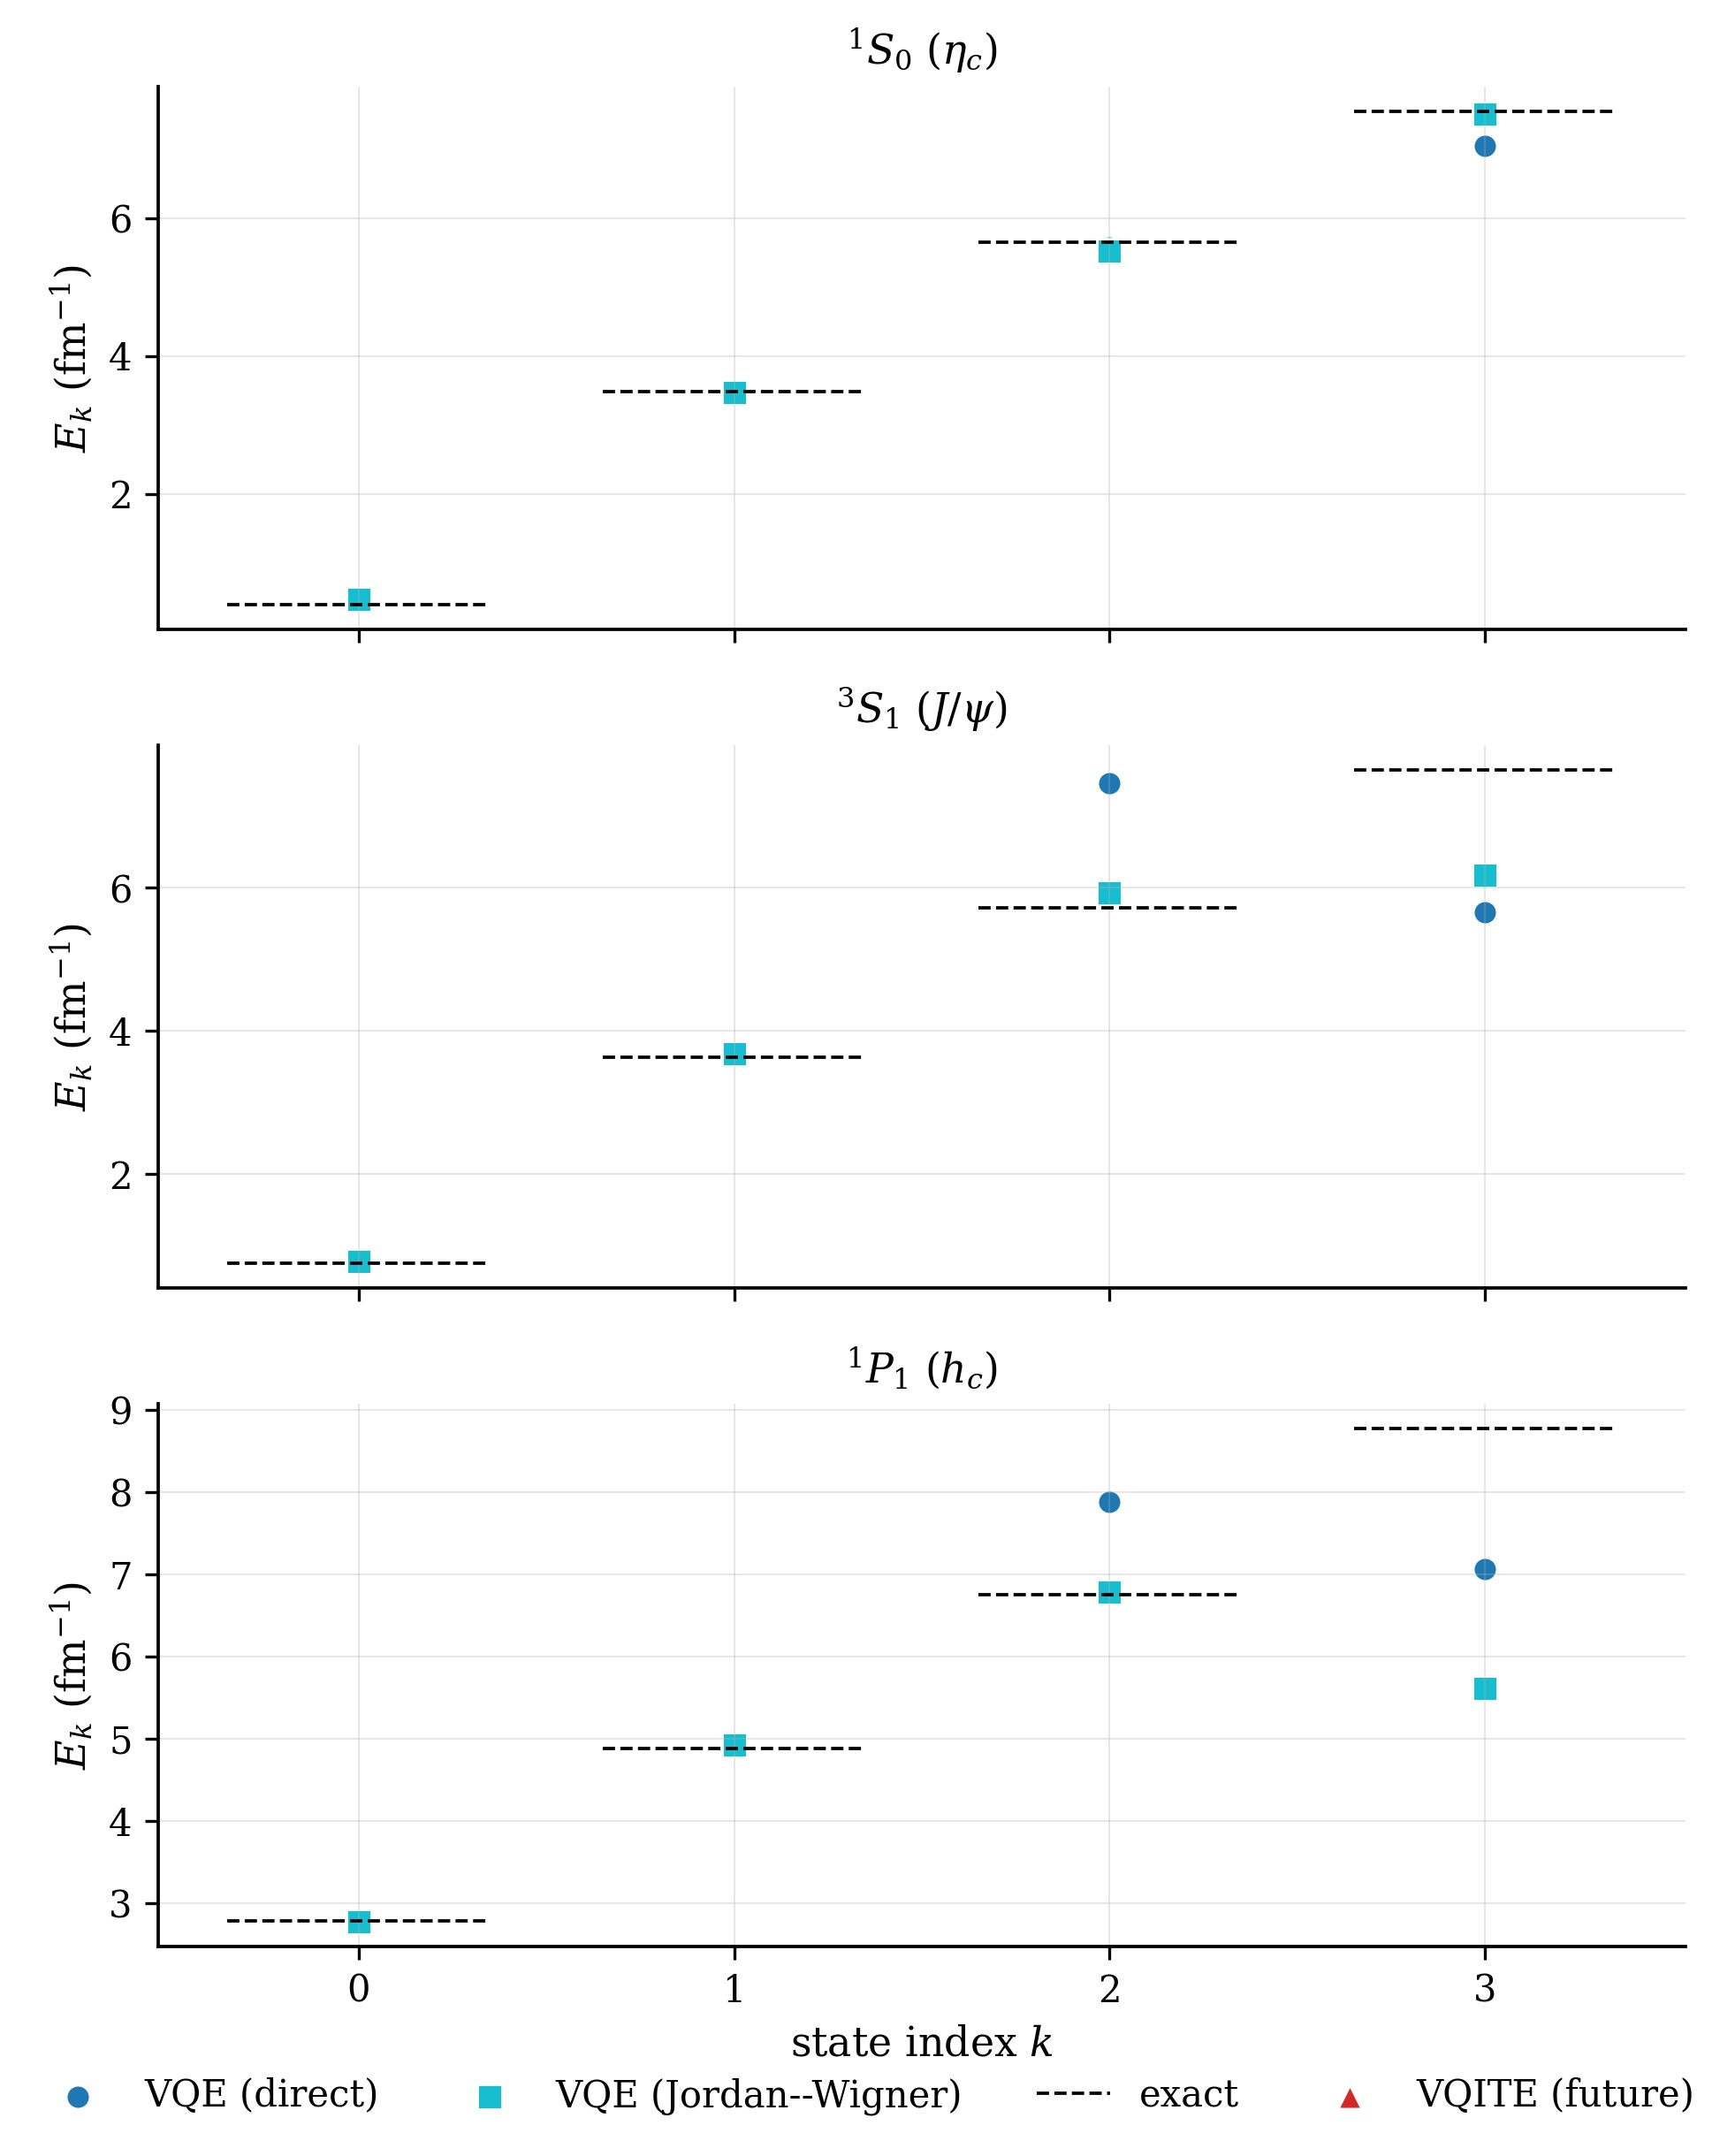
\includegraphics[width=\textwidth]{figures/excited_states.jpeg}
\caption{Energy-level diagram for the three channels. Black dashes mark
  the exact eigenvalues; coloured markers are the penalty-based VQE
  estimates in both encodings. The slot for VQITE excited states is
  preserved for follow-up work.}
\label{fig:excited}
\end{figure}

\Cref{fig:excited} shows the same information graphically. The ground
and first excited states are recovered with errors of at most
$\sim 0.08$~fm$^{-1}$ across all channels and both encodings. Higher
states ($k=2,3$) are more difficult: the penalty cost in
\cref{eq:penalised_H} stiffens the optimisation landscape as the
already-found subspace grows, and gradient-free COBYLA can converge to
the wrong eigenstate of the constrained problem. In several
${}^3S_1$ and ${}^1P_1$ entries the penalty method exchanges the
identities of $k=2$ and $k=3$ (e.g.\ VQE on ${}^3S_1$ assigns
$E_2 \approx 7.5$, near the exact $E_3 = 7.65$, and $E_3 \approx 5.7$,
near the exact $E_2 = 5.73$). VQE-JW is noticeably more reliable on
the third level for ${}^1S_0$ and ${}^1P_1$, though it inherits the
same $k=3$ degradation elsewhere.

% ──────────────────────────────────────────────────────────────────
\section{Noisy benchmark}
\label{sec:noisy}

We now switch the simulator backend to
\texttt{AerSimulator(noise\_model=make\_noise\_model($p$))} and re-run
the ground-state computation for each method at the five depolarising
rates listed in \cref{sec:results-setup}. \Cref{fig:noise-energy}
plots the absolute energy error against $p$ for the three channels;
\cref{fig:noise-fidelity} plots the fidelity. The Jordan--Wigner VQE
variant is omitted from the sweep, since its circuit class is similar
to the direct-encoding VQE and the qualitative noise response is the
same; the per-method noise behaviour discussed below applies to it as
well.

\begin{figure}[htbp]
\centering
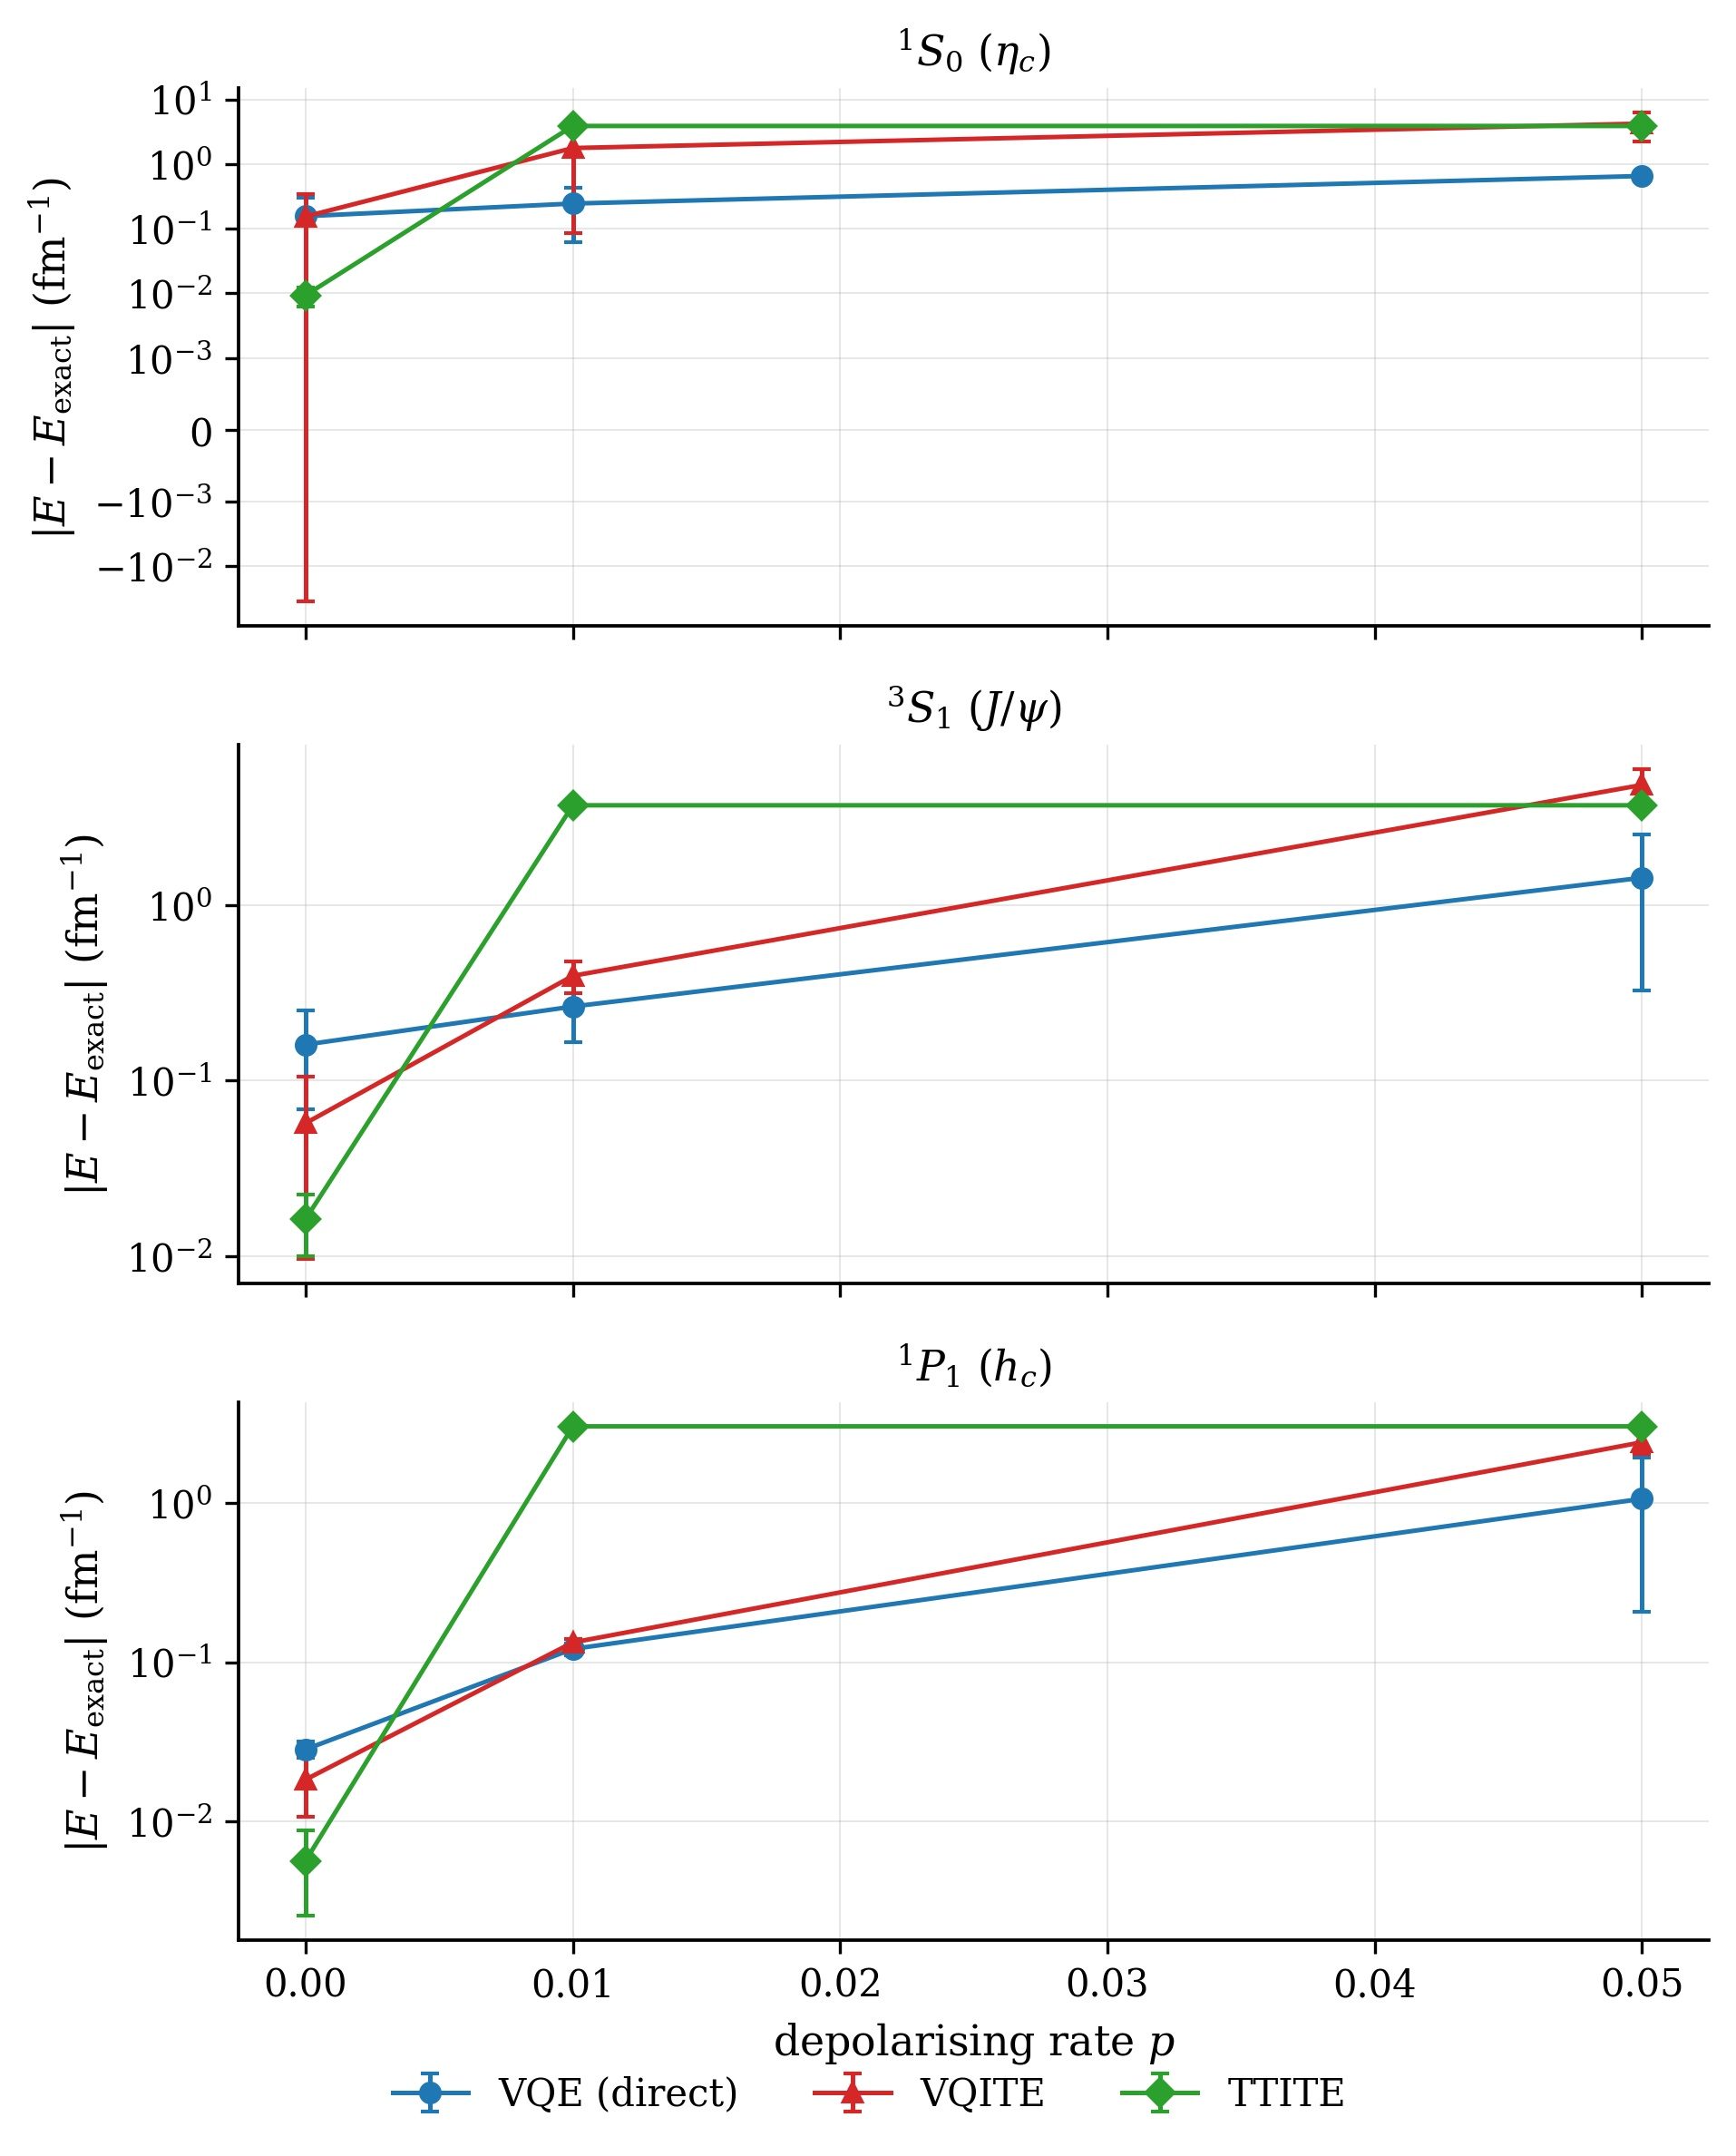
\includegraphics[width=\textwidth]{figures/noise_sweep_energy.jpeg}
\caption{Absolute energy error vs.\ depolarising rate $p$ for each
  channel. Error bars are the standard deviation over three repeats.
  The $y$-axis is symmetric-log to capture both the sub-$10^{-3}$
  noiseless regime and the $\mathcal{O}(1)$ degradation at $p = 0.05$.}
\label{fig:noise-energy}
\end{figure}

\begin{figure}[htbp]
\centering
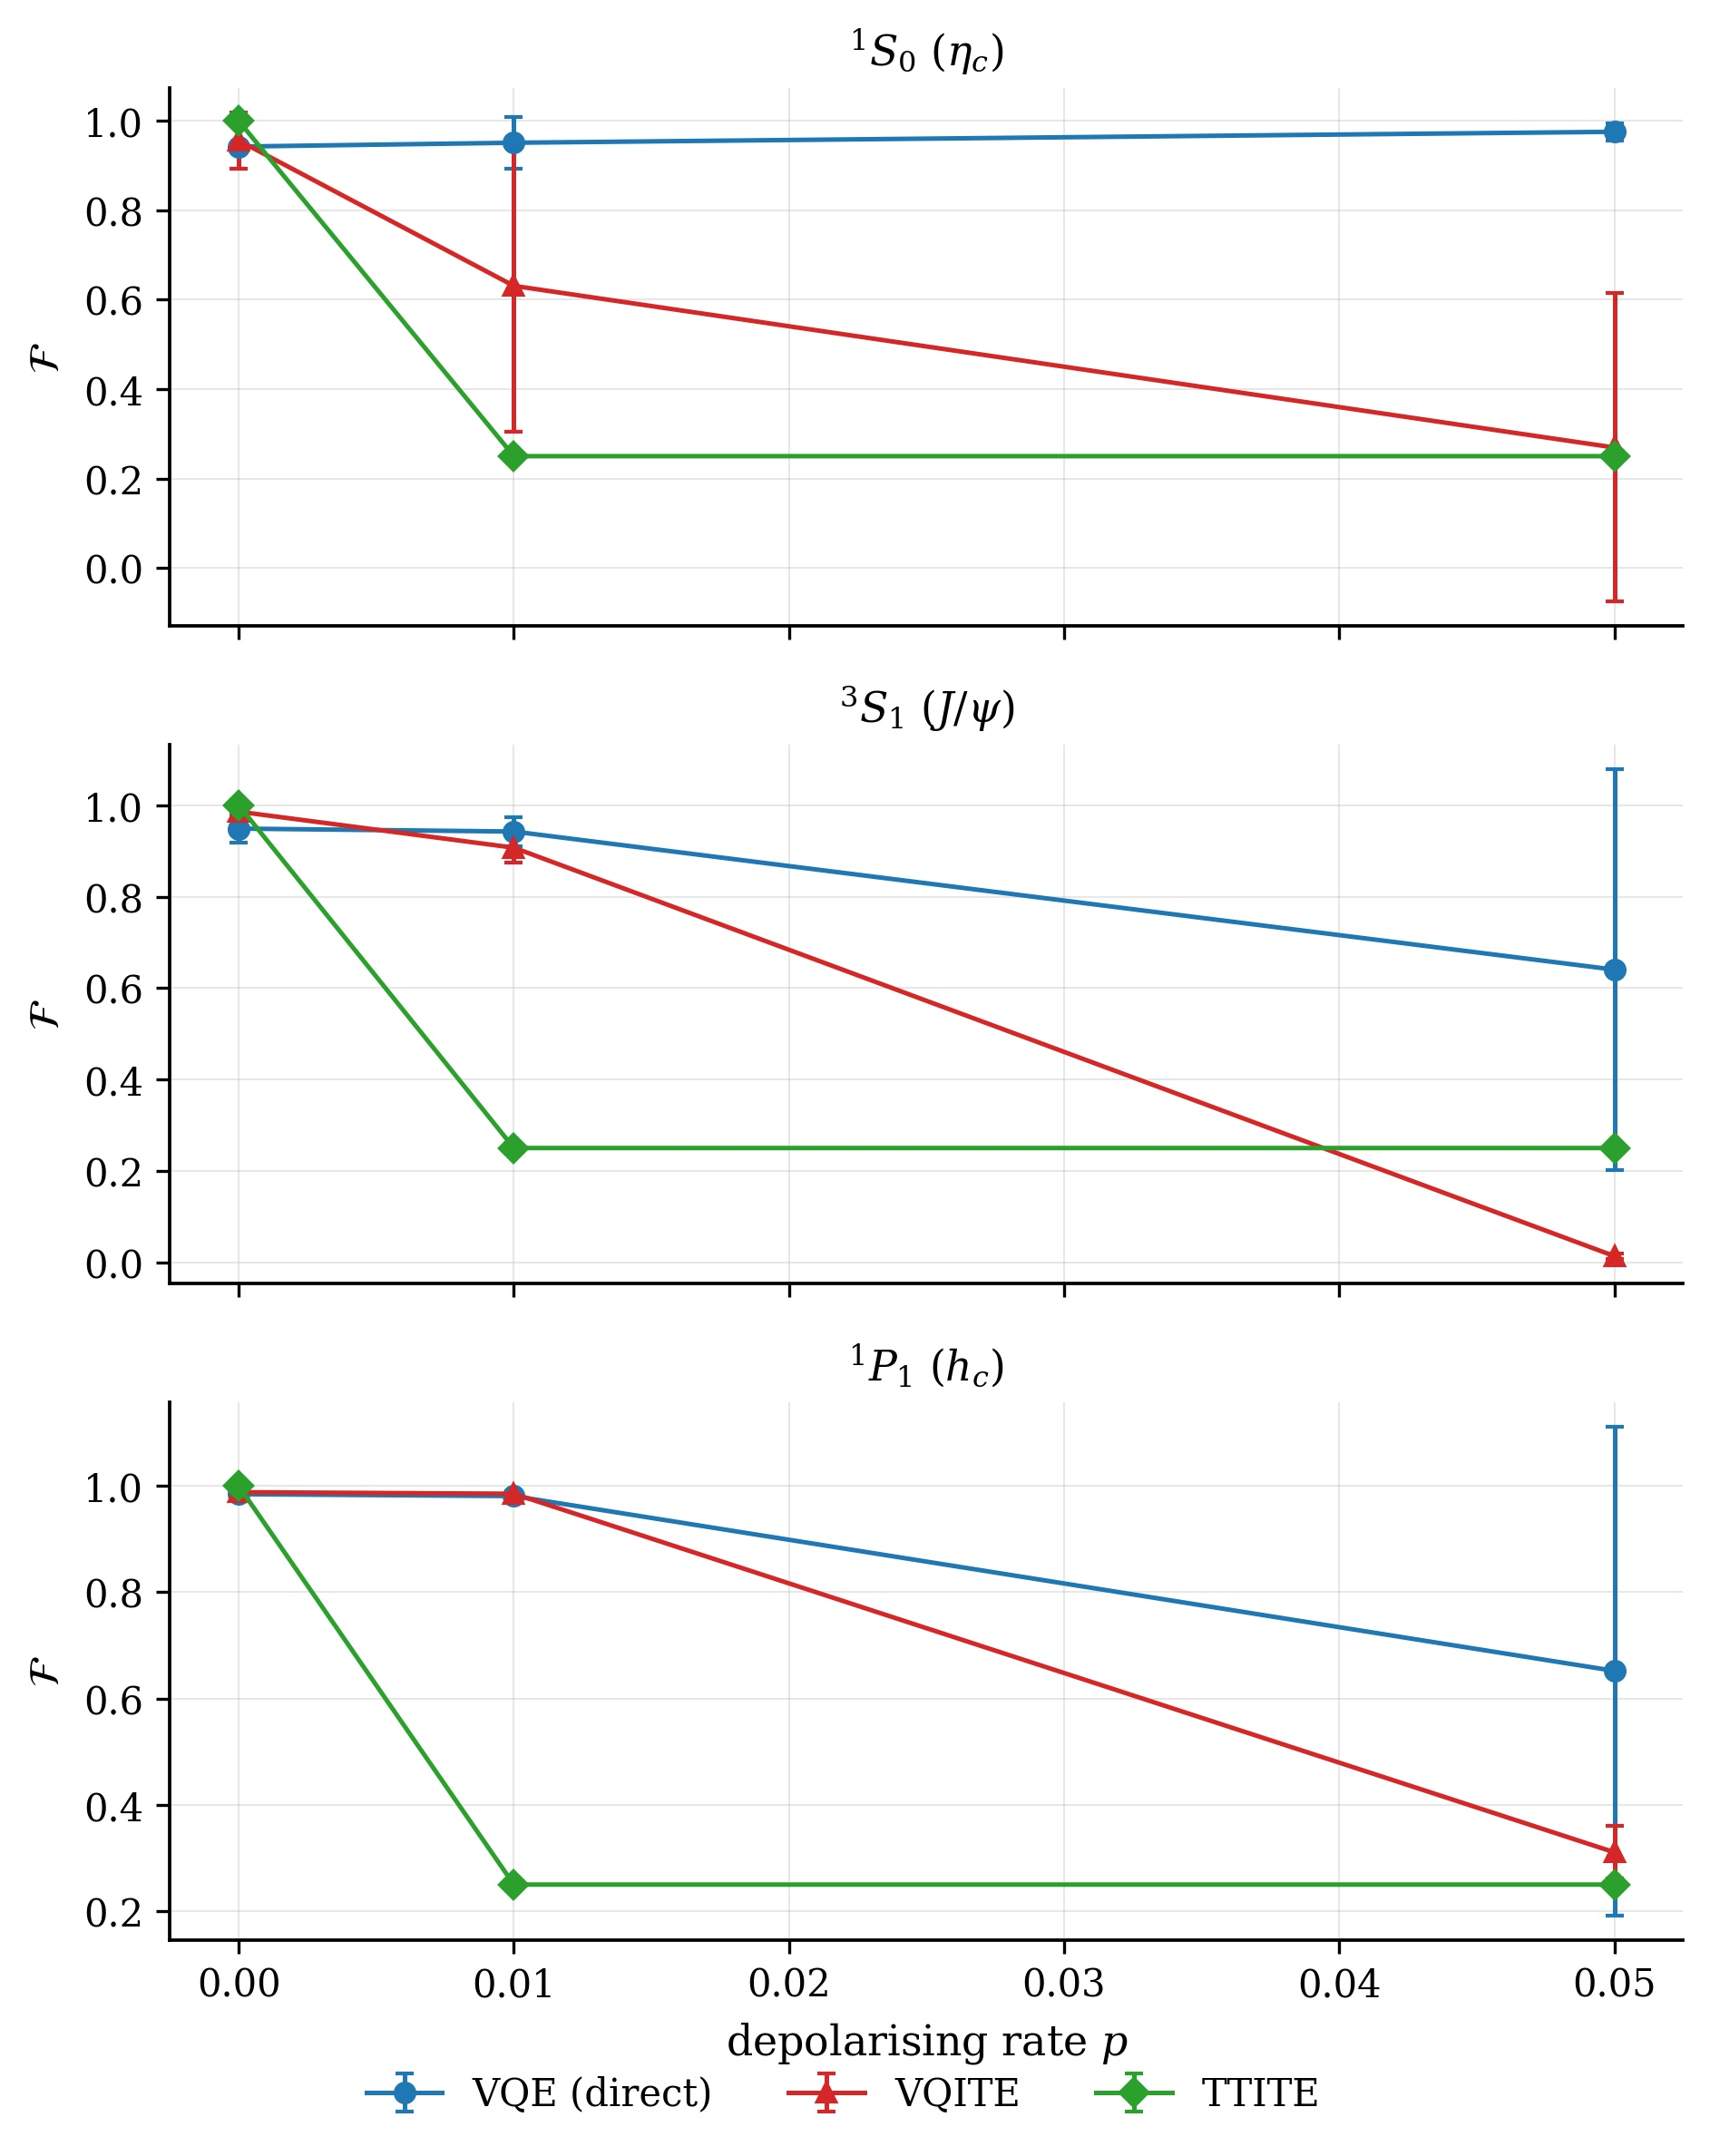
\includegraphics[width=\textwidth]{figures/noise_sweep_fidelity.jpeg}
\caption{Ground-state fidelity vs.\ depolarising rate $p$ for each
  channel. Error bars are the standard deviation over three repeats.}
\label{fig:noise-fidelity}
\end{figure}

The three algorithms degrade in qualitatively different ways. VQE is
the most resilient: its shallow ansatz (\cref{fig:woloshyn_ansatz}) is
exposed to only $\mathcal{O}(1)$ gates per energy evaluation, and the
gradient-free optimiser absorbs the resulting shot+gate noise into the
search. VQITE degrades faster because the metric tensor and
parameter-shift estimates of \cref{eq:metric_fd,eq:param_shift} both
require differences of noisy expectation values, so its effective
signal-to-noise ratio drops more sharply with $p$. TTITE collapses
catastrophically: with $\sim\!2{,}250$ sequential noisy gates over a
full Trotter trajectory and post-selection that cannot reject failed
LCU branches on real hardware, the work register relaxes toward the
maximally mixed state $\mathrm{Tr}(H)/4$, and the fidelity drops to
${\sim}\,0.25$ (random guessing in the 4-d Hilbert space) at any
non-zero noise rate.

% ──────────────────────────────────────────────────────────────────
\section{Summary}
\label{sec:results-summary}

In the noiseless regime all four methods reproduce the channel
eigenvalues, but they are not interchangeable: TTITE is essentially
exact (limited by simulation precision), VQE in either encoding is
limited by the chosen ansatz at the $\sim 10^{-2}$~fm$^{-1}$ level,
and VQITE accuracy is channel dependent because the metric tensor is
sensitive to the shape of the energy landscape. Under depolarising
noise the ranking inverts: VQE is the most resilient and TTITE the
most fragile, with the cross-over already at $p \lesssim 10^{-2}$.
These observations motivate the noise-mitigation strategies developed
in the next chapter.
